%
\documentclass[12pt]{article}

% The usual packages
\usepackage{fullpage}
\usepackage{breakcites}
\usepackage{setspace}
\usepackage{endnotes}
\usepackage{float}
\usepackage{amsmath}
\usepackage{amsfonts}
\usepackage{amssymb}
\usepackage{rotating}
\usepackage{dcolumn}
\usepackage{longtable}
\usepackage{microtype}
\usepackage{graphicx}
\usepackage{hyperref}
%\usepackage[usenames,dvipsnames]{color}
\usepackage{url}
\usepackage{natbib}
\usepackage{framed}
\usepackage{epigraph}
\usepackage{lipsum}
\usepackage[font=small,labelfont=sc]{caption}
\restylefloat{table}
\bibpunct{(}{)}{;}{a}{}{,}

% Set paragraph spacing the way I like
\parskip=0pt
\parindent=20pt

% Define mathematical results
\newtheorem{lemma}{Lemma}
\newtheorem{proposition}{Proposition}
\newtheorem{theorem}{Theorem}
\newtheorem{claim}{Claim}
\newenvironment{proof}[1][Proof]{\begin{trivlist}
\item[\hskip \labelsep {\bfseries #1}]}{\end{trivlist}}
\newenvironment{definition}[1][Definition]{\begin{trivlist}
\item[\hskip \labelsep {\bfseries #1}]}{\end{trivlist}}
\newenvironment{example}[1][Example]{\begin{trivlist}
\item[\hskip \labelsep {\bfseries #1}]}{\end{trivlist}}
\newenvironment{remark}[1][Remark]{\begin{trivlist}
\item[\hskip \labelsep {\bfseries #1}]}{\end{trivlist}}

% Set up fonts the way I like
\usepackage{tgpagella}
\usepackage[T1]{fontenc}
\usepackage[bitstream-charter]{mathdesign}

%% Set up lists the way I like
% Redefine the first level
\renewcommand{\theenumi}{\arabic{enumi}.}
\renewcommand{\labelenumi}{\theenumi}
% Redefine the second level
\renewcommand{\theenumii}{\alph{enumii}.}
\renewcommand{\labelenumii}{\theenumii}
% Redefine the third level
\renewcommand{\theenumiii}{\roman{enumiii}.}
\renewcommand{\labelenumiii}{\theenumiii}
% Redefine the fourth level
\renewcommand{\theenumiv}{\Alph{enumiv}.}
\renewcommand{\labelenumiv}{\theenumiv}
% Eliminate spacing around lists
\usepackage{enumitem}
\setlist{nolistsep}

% Create footnote command so that my name
% has an asterisk rather than a one.
\long\def\symbolfootnote[#1]#2{\begingroup%
\def\thefootnote{\fnsymbol{footnote}}\footnote[#1]{#2}\endgroup}

% Create the colors I want
\usepackage{color}
\definecolor{darkred}{RGB}{100,0,0}

\hypersetup{
 pdftitle={Practical Advice for Logistic Regression with a Small Sample}, % title
 pdfauthor={Kelly McCaskey and Carlisle Rainey}, % author
 pdfkeywords={logit}{probit}{logistic regression} {small sample} {bias}{MCMC}{Metropolis},
 pdfnewwindow=true, % links in new window
 colorlinks=true, % false: boxed links; true: colored links
 linkcolor=darkred, % color of internal links
 citecolor=darkred, % color of links to bibliography
 filecolor=darkred, % color of file links
 urlcolor=darkred % color of external links
}

% enable comments in pdf
\newcommand{\kelly}[1]{\textcolor{blue}{#1}}
\newcommand{\carlisle}[1]{\textcolor{magenta}{#1}}


\begin{document}

\begin{center}
{\Large Practical Advice for Logistic Regression with a Small Sample}\\\vspace{2mm}
{\large Penalized Maximum Likelihood and Metropolis Sampling\symbolfootnote[1]{We thank [people] for making their data available to us. The analyses presented here were conducted with \texttt{R} 3.1.0. All data and computer code necessary for replication are available at [GitHub url].}}\\\vspace{2mm}


\vspace{10mm}

Kelly McCaskey\symbolfootnote[2]{Kelly McCaskey is a Ph.D. student in the Department of Political Science, University at Buffalo, SUNY, 520 Park Hall, Buffalo, NY 14260 (\href{mailto:kellymcc@buffalo.edu}{kellymcc@buffalo.edu}).}

\vspace{3mm}

Carlisle Rainey\symbolfootnote[3]{Carlisle Rainey is Assistant Professor of Political Science, University at Buffalo, SUNY, 520 Park Hall, Buffalo, NY 14260 (\href{mailto:rcrainey@buffalo.edu}{rcrainey@buffalo.edu}).}
\end{center}

\vspace{10mm}

% Abstract
{\centerline{\textbf{Abstract}}}
\begin{quote}\noindent
When used in small samples, logistic regression models present two problems. First, the estimates are noticeably biased away from zero, as much as 25 percent in plausible scenarios. Secondly, the sampling distributions are not well-approximated by a normal distributions, which makes computing confidence intervals challenging, especially for quantities of interest, such as first-differences or risk-ratios. As a solution to these problems, we first (re)introduce political scientists to Firth's penalty, which removes much of the bias from the usual estimator. Secondly, we explain how researchers can use a random walk Metropolis algorithm to obtain Clarify-like simulations from the posterior distribution to obtain confidence intervals for quantities of interest.
 \end{quote}


% Remove page number from first page
\thispagestyle{empty}

% Start main text
\newpage
\doublespace

% three figures
% 1. simulation results
% 2. coefficient estimates
% 3. qi ci

\section*{Introduction}

Asymptotically, the maximum likelihood estimator for the coefficients of a logistic regression model is centered at the true coefficient and normally distributed. However, in small samples, the sampling distribution is neither centered at the true coefficient nor normally distributed. Estimating logistic regression models with small data sets leads to estimates that are substantially biased away from zero with sampling distributions that are skewed away from zero. 

Thus, logistic regression with a small sample presents the researcher with two problems: 
\begin{enumerate}
\item How can she correct the potentially substantial bias in the coefficient estimates? 
\item How can she obtain accurate confidence intervals without relying on the assumption of normality, especially for quantities of interest?
\end{enumerate}
	19
In the typical situation, the researcher models the probability of an event as $\text{Pr}(y_i) = \text{Pr}(y_i = 1~|~ X_i) = \dfrac{1}{1 + e^{-X_i\beta}}$, where $y$ is a vector of binary outcomes, $X$ is a matrix of explanatory variables and an intercept, and $\beta$ is a vector of model coefficients. Using this model, it is straightforward to calculate the likelihood function 

\begin{equation}\nonumber
\text{Pr}(y | \beta) = L(\beta | y) = \displaystyle \prod_{i = 1}^n \left[\left( \dfrac{1}{1 + e^{-X_i\beta}}\right)^{y_i}\left( \dfrac{1}{1 + e^{-X_i\beta}}\right)^{1 - y_i}\right]\text{.}
\end{equation}

\noindent As usual, one can take the natural logarithm of both sides to calculate the log-likelihood function 

\begin{equation}\nonumber
\log L(\beta | y) = \displaystyle \sum_{i = 1}^n \left[y_i \log \left( \dfrac{1}{1 + e^{-X_i\beta}}\right) + (1 - y_i) \log \left( \dfrac{1}{1 + e^{-X_i\beta}}\right)\right].
\end{equation}

%\noindent and take the derivatives of the log-likelihood function to obtain the score function
%
%\begin{equation}\nonumber
%\dfrac{\partial \log L(\beta | y)}{\partial \beta} = \displaystyle \sum_{i = 1}^n\left(y_i - \dfrac{1}{1 + e^{-X_i\beta}}\right)X_i\text{.}
%\end{equation}

The researcher can obtain the maximum likelihood estimate $\hat{\beta}^{mle}$ by finding the vector $\beta \in \mathbb{R}^{k + 1}$ that maximizes $\log L$. However, as noted above, this estimate is biased, so the $E(\hat{\beta}^{mle}) \neq \beta^{true}$.

\section*{Correcting the Bias}

The statistics literature offers a simple solution to the problem of bias. \citet{Firth1993} suggests penalizing the usual likelihood function $L(\beta | y)$ by a factor equal to the square root of the determinant of the information matrix $I(\beta)|^\frac{1}{2}$, which yields a ``penalized'' likelihood function $L^*(\beta | y) = L(\beta | y)|I(\beta)|^\frac{1}{2}$.\footnote{It turns out that this penalty is equivalent to Jeffreys' (\citeyear{Jeffreys1946}) prior for the logistic regression model (\citealt{Firth1993}, \citealt{Poirier1994}).} Taking logs yields the penalized log-likelihood function.
\begin{equation}\nonumber
\log L^*(\beta | y) = \displaystyle \sum_{i = 1}^n \left[y_i \log \left( \dfrac{1}{1 + e^{-X_i\beta}}\right) + (1 - y_i) \log \left( \dfrac{1}{1 + e^{-X_i\beta}}\right)\right] + 0.5 \log |I(\beta)|.
\end{equation}
Then the researcher can obtain the \emph{penalized} maximum likelihood estimate $\hat{\beta}^{pmle}$ by finding the vector $\beta \in \mathbb{R}^{k + 1}$ that maximizes $\log L^*$. \citet{Firth1993} shows that $\hat{\beta}^{pmle}$ is much less biased than $\hat{\beta}^{mle}$. The penalized maximum likelihood estimate is easy to calculate in R using the \texttt{logistf()} function in the \texttt{logistf} package. See the Online Appendix for an example.

To demonstrate the substantial bias of $\hat{\beta}^{mle}$ and the near unbiasedness of $\hat{\beta}^{pmle}$, we calculate the bias (\%) as the sample size, proportion of events, and number of explanatory variables vary.\footnote{The true data generating process is always $\Pr(y_i = 1) = \frac{1}{1 + e^{-X_i \beta}}$, where $i \in 1, 2,..., n$ and $X_i \beta = \beta_{cons} + 0.25 x_1 + \sum_{j = 2}^k 0.15 x_j$. Each fixed $x_j$ is drawn from a normal distribution with mean of zero and standard deviation of one. The simulation controls the size of the sample by varying $n$, the number of explanatory variables by varying $k$, and the proportion of events by varying $\beta_{cons}$. The expected values of the MLE  and PMLE of the coefficient for $x_1$ are calculated by simulating 10,000 data sets, calculating the MLE and PLME for each data set, and then finding the average of the MLE and PMLE across the 10,000 data sets. The bias (\%) is calculated the average estimate divided by the true value, which is 0.25 in our simulations.} Figure \ref{fig:bias-sims} shows the results. Across the range of the parameters of our sample, the bias of the MLE varies from about 50\% (19\% events, 9 predictors, 50 observations) to around 2\% (50\% events, 3 predictors, 200 observations). Any bias in the PMLE, on the other hand, is barely noticeable.

\begin{figure}[H]
\begin{center}
\includegraphics[width = \textwidth]{bias-sims.png}
\caption{This figure demonstrates the substantial bias of $\hat{\beta}^{mle}$ and the near unbiasedness of $\hat{\beta}^{pmle}$. Notice that when $N = 50$, the bias of $\hat{\beta}^{mle}$ away from zero is about 40\% or more if events are relatively uncommon (e.g., 19\% events) or the researcher uses several explanatory variables (e.g., 9). However, notice that $\hat{\beta}^{pmle}$ is essentially unbiased regardless of the small size, proportion of events, and number of explanatory variables.}\label{fig:bias-sims}
\end{center}
\end{figure}

\section*{Accounting for the Skewed Sampling Distribution}

The usual method of obtaining standard errors for maximum likelihood estimates is to assume a multivariate normal sampling distribution for the parameter vector $\beta$ and obtain the $(i, j)$ entry of the covariance matrix $I(\hat{\beta}^{mle})^{-1} = \Sigma^{[\hat{\beta}^{mle}]}$ by calculating the curvature around the maximum likelihood using $\frac{\partial^2 \log L(\beta | Y)}{\partial \beta_i \partial \beta_j}$. This approximation also works for penalized maximum likelihood, so that $\Sigma^{[\hat{\beta}^{pmle}]}_{i,j} = \frac{\partial^2 \log L^*(\beta | Y)}{\partial \beta_i \partial \beta_j}$. However, this method only works well for large samples--with small samples, the researcher must take into account the skewness in the sampling distribution \citep{Barndorff-NielsonCox1994}.

If the researcher is only interested in confidence intervals for the logistic regression coefficients, then she can obtain these through the profile likelihood. See \citet{McCullaghNelder1989} for the details. The profile likelihood confidence intervals for the parameters are easily produced using the \texttt{logistf()} function in the R package \texttt{logistic}. See the Online Appendix for an example.

However, researchers are not usually directly interested in logistic regression coefficients. Instead, they are interested in \emph{functions} of the coefficients, such as first-differences and risk-ratios \citep{King1989, KingTomzWittenberg2000}. However, ``Clarify-like'' simulation \citep{TomzWittenbergKing2003} or ``informal Bayesian'' simulation \citep{GelmanHill2006} typically relies on the asymptotic posterior, which might be a poor approximation in small samples. However, rather than relying on an inaccurate normal approximation, researchers can use a Metropolis algorithm to directly sample from the actual posterior.

Notice that Firth's penalty \citep{Firth1993} is equivalent to Jeffreys' prior for the parameters of the logistic regression model \citep{Jeffreys1946, Poirier1994}, so the $p(\beta) = I(\beta)|^\frac{1}{2}$. This implies that the penalized likelihood $L^*$ is proportional to the posterior distribution for the coefficients, so that 
\begin{equation}\label{eqn:post}
p(\beta | y) \propto \sum_{i = 1}^n \left[y_i \log \left( \dfrac{1}{1 + e^{-X_i\beta}}\right) + (1 - y_i) \log \left( \dfrac{1}{1 + e^{-X_i\beta}}\right)\right] + 0.5 \log |I(\beta)|.
\end{equation}
The Metropolis algorithm \citep{Metropolisetal1953, Gelmanetal2013} allows researchers to sample directly from this posterior distribution using Markov chains. She can construct each chain as follows:
\begin{enumerate}
\item Choose an arbitrary starting point $\tilde{\beta}^{[0]}$ to serve as the starting point for the sampler.  We recommend random, over-dispersed starting values. This proves especially helpful when monitoring convergence using multiple chains run in parallel. 
\item Choose a proposal distribution from which to generate samples. We recommend the multivariate normal distribution with variance $\Sigma^{[\hat{\beta}^{mle}]}$.
\item For each subsequent iteration $i$ of the chain:
	\begin{enumerate}
	\item Simulate a \underline{p}roposed sample $\tilde{\beta}^{p} \sim N(\tilde{\beta}^{[i - 1]}, \Sigma^{[\hat{\beta}^{mle}]})$.
	\item Calculate the acceptance ratio $\alpha = \frac{L^*(tilde{\beta}^{p} | y)}{L^*(tilde{\beta}^{[0]} | y)} = \frac{p(\tilde{\beta}^{p} | y)}{p(\tilde{\beta}^{[0]} | y)}$.
	\item Sample a value $u$ from a uniform distribution from zero to one. Set $\tilde{\beta}^{[i]} = \tilde{\beta}^{p}$ if $\alpha > u$. If $\alpha \leq u$, then set $\tilde{\beta}^{[i]} = \tilde{\beta}^{[i - 1]}$.
	\end{enumerate}
\end{enumerate} 

Each chain eventually converges to the posterior distribution. However, this convergence might require a large number of iterations. In practice, we recommend that researchers (1) run multiple chains (either in parallel or sequentially), (2) discard the first half of the chain as a ``burn-in'' period, and (3) monitor convergence of the second-half using \citet{GelmanRubin1992}'s $\hat{R}$ statistic. If the starting values for each chain are over-dispersed, then an $\hat{R}$ near one (e.g., 1.02) indicates convergence. Once the researcher is satisfied that the chains have converged, she may combine the chains and treat the simulations as a large number of independent simulations from the posterior distribution and proceed as recommended by \citet{KingTomzWittenberg2000}. To make this simulation easy, we have written an R function \texttt{logit.jeffreys()} in the R package \texttt{pppd} available on GitHub. For an example, see the Online Appendix.

\section*{Replication of Weisiger (2014)}
\citet{Weisiger2014} explains that conquerors in conventional wars cannot expect to win over the defeated population. Additionally, he describes how sometimes violence continues after the official end of the war in the form of guerrilla warfare instead. Weisiger argues that if resistance occurs, it will be where conditions are favorable for insurgency, such as, difficult terrain, the size and concentration of the occupying force, or if there remains a pre-war leader for potential insurgents to rally around. He hypothesizes that there will be a greater chance of resistance when the pre-conflict political leader ``remains at large in the conquered country" (p. 8).

Weisiger's sample consists of 35 observations so the original analysis uses multivariate linear probability regressions to test his hypotheses. He does so in order to avoid problems with separation and biases that may occur with his small sample if he were to use the standard logit or probit analysis. He acknowledges the limitations to using multivariate linear probability regressions in this situation by noting that the method introduces the possibility of estimating non-meaningful predicted probabilities outside the [0, 1] range. We replicate his results and are able to correct the bias of the coefficient estimates and account for the skewed sampling distribution by using the Metropolis algorithm to sample directly from the posterior distribution and using those simulations in penalized maximum likelihood estimation (PMLE). 

The use of a logit analysis implies that we are more interested in the functions of the coefficients rather than the coefficients themselves, so we calculated the first differences for his hypothesis about the presence of the pre-conquest political leader. To do so, we evaluated the difference in the probability of resistance from a situation where there a pre-conquest leader did not remain to a situation where one did remain. We then set the Polity score of the Conqueror to 10, a full democracy, and the rest of the variables at their medians.\footnote{These include: the natural log of the intercapital distance, the type of terrain, the density of the occupying force and the conquered country's per capita GDP.}  We did this for the standard MLE with asymptotic approximation, PMLE with asymptotic approximation, and PMLE with MCMC sampling. The resulting first differences and 90\% confidence intervals, shown in Figure \ref{fig:coord-fd}, demonstrate how PMLE with MCMC sampling provides an unbiased estimate and an appropriately skewed distribution. Using PMLE with MCMC sampling provides us with a $p$-value of 0.01, indicating that we can be confident in both our rejection of the null hypothesis and the accuracy of our coefficients when using the more appropriate logistic regression instead of multivariate linear probability analysis.\footnote{PMLE with asymptotic approximation yields a $p$-value of 0.03, MLE with a $p$-value of 0.03, and OLS with a $p$-value of 0.009.} 

\begin{figure}[H]
\begin{center}
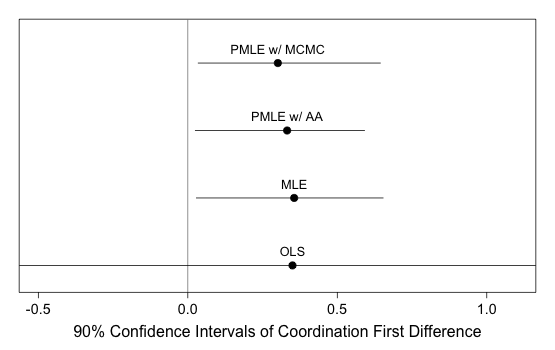
\includegraphics[width = \textwidth]{weisiger-coordfd.png}
\caption{This figure demonstrates the first difference when we move from a scenario in which no pre-conquest leader remains to a situation in which the pre-conquest leader serves as a post-conquest rallying point, using a multivariate linear probability model, MLE, PMLE with asymptotic approximation, and PMLE with MCMC sampling.}\label{fig:coord-fd}
\end{center}
\end{figure}

By replicating \citet{Weisiger2014}, we demonstrate an appropriate way to use logistic regression with small samples. His original study uses multivariate linear probability regressions on his sample of 35 observations to avoid problems with separation and bias. Using MCMC sampling directly from the posterior, we show that the author would be able to make a stronger case for his argument by obtaining more precise estimates by correcting the bias on the coefficients and the skew of the sampling distributions. 

\singlespace 
\newpage
\normalsize
\bibliographystyle{apsr_fs}
% \bibliography{/Users/carlislerainey/Dropbox/papers/bibliography/bibliography.bib}
\bibliography{/Users/kellymccaskey/Dropbox/Projects/bibliography/bibliography.bib}

\newpage
\begin{appendix}
\begin{center}
{\LARGE Online Appendix}\\
{\large Practical Advice for Logistic Regression with a Small Sample}\\\vspace{2mm}
\end{center}


\section{Using \texttt{logistf()} to Calculate the PMLE and Confidence Interval}

\section{Using \texttt{logit.jeffreys()} to Obtain Posterior Simulations Using Jeffreys' Prior}

\end{appendix}


\end{document}